%!TEX root = ./template-skripsi.tex
%-------------------------------------------------------------------------------
%                            	BAB IV
%               		KESIMPULAN DAN SARAN
%-------------------------------------------------------------------------------

\chapter{HASIL DAN PEMBAHASAN}

\section{Pengolahan data citra input}

Untuk optimal nya pendeteksia luka, maka piksel 
yang dipindai dikurangi dengan memotong citra yang 
dipindai. Pemotongan ini dilakukan dengan menggunakan 
program GIMP(\textit{GNU Image Manipulation Program}) dan 
memakai fungsi \textit{crop} 

Langkah selanjutnya dalam pengolahan citra ini dimulai dengan 
membaca citra nya dalam bentuk hitam putih(\textit{grayscale}). 
Proses pengolahan data citra input menggunakan \textit{imread} yang merupakan 
fungsi yang di-\textit{import} dari CV2
\begin{figure}[H]
	\centering
	\begin{lstlisting}[language=Python, basicstyle=\tiny]
		import cv2 as cv2

		gambar = cv2.imread(image, cv2.IMREADGRAYSCALE)
	\end{lstlisting}
	\caption{Kode untuk membaca citra}
	\label{kode:imread}
\end{figure}

\section{Deteksi Keliling Menggunakan \textit{Border Following}}

Citra yang sudah dimasukkan akan diolah oleh program 
\textit{border following}. Metode ini akan membaca citra 
dalam bentuk citra biner yang hanya terisi 0 dan 1. 
Dibentuklah kode sebagai berikut yang mengikuti kode 
dibuat oleh Hafizhun Alim(\cite{Hafizhun}) pada skripsi-nya 
yang berjudul "\textit{Fish Movement Tracking Menggunakan 
Metode Gaussian Mixture Models (GMM) dan Kalman Filter}".
\begin{figure}[H]
	\centering
	\begin{lstlisting}[language=Python, basicstyle=\tiny]
		def border_following(self, img, start, previous):

			pointer_one = previous
			pointer_three = start
			contour = []

		# Step 3.1 Move clockwise
		count = 0
		while img[pointer_one[0]][pointer_one[1]] == 0:
			# If the starting pixel is a single pixel dot
			if count > 7:
				img[pointer_three[0]][pointer_three[1]] = 4
				contour.append(np.array([[pointer_three[1] - 1, pointer_three[0] - 1]]))
				return np.array(contour)
					
			position, next_pointer = self.next_pointer_position(pointer_one, pointer_three, 1)
			pointer_one = next_pointer
			count += 1
	
	\end{lstlisting}
\end{figure}
\begin{figure}[H]
	\centering
	\begin{lstlisting}[language=Python, basicstyle=\tiny]
        # Step 3.2
        pointer_two = copy.copy(pointer_one)

        counter = 0
        while True:
            # Step 3.3 Move counter clockwise
            # First, move pointer one time in counter-clockwise direction
            position, next_pointer = self.next_pointer_position(pointer_two, pointer_three, 2)
            pointer_two = next_pointer
            while img[pointer_two[0]][pointer_two[1]] == 0:
                position, next_pointer = self.next_pointer_position(pointer_two, pointer_three, 2)
                pointer_two = next_pointer
            pointer_four = pointer_two
			
		# Step 3.4 Assign NBD
		# rows or i represent y-axis
		# cols or j represent x-axis
		# the coordinate are inverted because we wanted to return a set of (x, y) points, not (y, x)
		# we use 2 and 4 (-2) since we only extract outer border
		nbd_coordinate = copy.copy(pointer_three)
		if img[nbd_coordinate[0]][nbd_coordinate[1] + 1] == 0:
			img[nbd_coordinate[0]][nbd_coordinate[1]] = 4
		elif img[nbd_coordinate[0]][nbd_coordinate[1] + 1] != 0 and img[nbd_coordinate[0]][nbd_coordinate[1]] == 1:
			img[nbd_coordinate[0]][nbd_coordinate[1]] = 2
            contour.append(np.array([[nbd_coordinate[1] - 1, nbd_coordinate[0] - 1]]))

            # Step 3.5 Determine new pointer or break
            if pointer_four[0] == start[0] and pointer_four[1] == start[1]:
                if pointer_three[0] == pointer_one[0] and pointer_three[1] == pointer_one[1]:
                    break
            pointer_two = copy.copy(pointer_three)
            pointer_three = copy.copy(pointer_four)

            counter += 1

        return np.array(contour)
	\end{lstlisting}
	\caption{Kode border following}
	\label{kode:border following}
\end{figure}

setelah jalannya program diatas, didapatkan 
hasil contour sebagai berikut
\begin{figure}[H]
	\centering
	\begin{subfigure}{.3\textwidth}
		\centering
		\includegraphics[keepaspectratio, width=3cm]{SourceCode/dataset/luka_merah/33.jpg}
		\caption{Sumber citra}
	\end{subfigure}
	\begin{subfigure}{.4\textwidth}
		\centering
		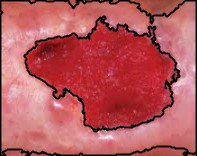
\includegraphics[keepaspectratio, width=3cm]{gambar/Bab4/Luka_merah_interpolasi.jpg}
		\caption{Hasil \textit{border following}}
	\end{subfigure} 
	\caption{Hasil pindai \textit{border following}}
\end{figure}
Dalam pendeteksiannya, metode ini akan menghasilkan 
lebih dari daerah dan terkadang mendeteksi daerah 
yang hanya memiliki satu titik koordinat. Untuk membuang 
daerah yang pasti bukan daerah luka, maka penulis 
hanya menggambar daerah yang memiliki 50 titik.


\section{Penghalusan menggunakan Interpolasi Global}

Dari hasil \textit{border following}, akurasi dari 
pindaian citra masih kasar dan belum 100$\%$ kepada 
\textit{ground truth}. Untuk membantu ini, penulis 
menggunakan \textit{Global Interpolation} yang ada 
di buku NURBS(\cite{PiegTill96}).

Penulis tidak menggunakan interpolasi lokal dikarenakan 
kurang mampunya penulis untuk mengerti cara penghitungan 
interpolasi lokal. Banya variabel yang penulis kurang tangkap 
seperti pada rumus(\ref{rumus:localbicubic}), di mana memiliki 
dua jenis \textit{knot vector} yang penulis tidak tahu 
perbedaannya.

Dimulai dengan rumus utama akan menggunakan 
algoritma(\ref{algoritma:globalinterpolation}). 
Algoritma ini akan membentuk kode sebagai berikut
\begin{figure}[H]
	\centering
	\begin{lstlisting}[language=Python, basicstyle=\tiny]
		def GlobalCurveInterpolation(Point, degree):
			Knot = GlobalInterpolation.ChordLength(Point)
			KnotVector = GlobalInterpolation.knotGlobalCurve(Knot, degree)
			nurb = np.empty([len(Point), len(Point)])
			for x in range(len(Point)):
				for y in range(len(Point)):
					nurb[x,y] = GlobalInterpolation.N(Knot[x], y, degree, KnotVector)

			#making sure the last array
			nurb[len(Point)-1,len(Point)-1] = 1.0

		
			hasil = np.dot(np.linalg.pinv(nurb), Point)

			return hasil
	\end{lstlisting}
	\caption{Kode Global Interpolation}
	\label{kode:GlobalInterpolation}
\end{figure}
Dari kode di atas, terdapat beberapa fungsi 
dari \textit{class} GlobalInterpolation yang 
akan dijelaskan sebagai berikut

Dalam interpolasi, menentukan titik-titik kurva 
membutuhkan \textit{knot}. \textit{Knot} dapat 
ditentukan dengan perata-rataan memakai fungsi 
\textit{numpy} yaitu np.linspace(0,1,len(Point)).
Ada juga metode lain yang memastikan kurva lebih 
stabil yaitu menggunakan \textit{chord length} 
menggunakan algoritma(\ref{algoritma:chordlength}).
\begin{figure}[H]
	\centering
	\begin{lstlisting}[language=Python, basicstyle=\tiny]
		def ChordLength(koordinat = np.array([0,0])):
			knot = np.empty([len(koordinat)],dtype=float)
			knot[0] = 0
			totalJarak = 0

			#d / total jarak
			for i in range(len(koordinat)):
				if(i>0):
					jarak = np.linalg.norm(koordinat[i-1] - koordinat[i])
					totalJarak += jarak
					knot[i] = totalJarak
		
			#knotkord
			for i in range(len(koordinat)):
				knot[i] = knot[i]/totalJarak

			#return as KnotVector, group of knots, 1d array
        	return np.array(knot)
	\end{lstlisting}
	\caption{Kode \textit{chord length}}
	\label{kode:chordlength}
\end{figure}

Setelah mendapatkan knot, langkah selanjutnya 
adalah membuat \textit{knot vector}. Kode untuk 
\textit{knot vector} akan dibentuk mengikuti 
algoritma(\ref{algoritma:knotvektor})
\begin{figure}[H]
	\centering
	\begin{lstlisting}[language=Python, basicstyle=\tiny]
		def knotGlobalCurve(knots = np.array([0]), degree=0):

			KnotVector = np.empty([len(knots) + degree + 1])
			for i, val in enumerate(KnotVector):
				if(i <= degree): KnotVector[i] = 0 
				elif(i >= len(KnotVector) - degree-1): KnotVector[i] = 1
				else:
					knotvector = 0.0
					for ii in range(i-degree, i):
						knotvector += knots[ii]
					KnotVector[i] = knotvector/degree

			#return as 1d array
			return KnotVector
	\end{lstlisting}
	\caption{Kode knot vector}
	\label{kode:knotvector}
\end{figure}

Dan metode utama yang dijalankan secara rekursif, 
yaitu rumus dasar interpolasi yang dilambangkan 
sebagai N di buku \textit{NURBS}. Dalam pembuatannya, 
penulis agak kesulitan dalam mendapatkan hasil yang 
ditujukan oleh buku. Masalah yang pertama dihadapi 
adalah membuat 0/0 menjadi 0. yang penulis pertama 
kali lakukan adalah mengecek penyebut merupakan 0 maka 
hasilnya akan 0. Metode ini menghasilkan nilai yang salah 
pada baris awal dan terakhir dan membuat kolom tengah 
menjadi 1 semua. Lalu, karena penyebut terjadi operasi 
pengurangan, pengecek nya diubah dengan apabila variabel 
kiri sama dengan yang kanan. Setelah pengetesan hampir 
semua nya benar kecuali angka terakhir, yang seharusnya 1 
menjadi 0, di sini penulis memaksa angka matriks terakhir 
menjadi 1. Berikut adalah kode untuk rumus dasar mengikuti
algoritma(\ref{algoritma:spline}).
\begin{figure}[H]
	\centering
	\begin{lstlisting}[language=Python, basicstyle=\tiny]
		def N(knot = 0.0, i = 0 , degree = 0, KnotVector = np.array([0])):

			#Basis function that used to count N in interpolation

			if (degree == 0):
				#
				return 1.0 if (KnotVector[i] <= knot < KnotVector[i + 1]) else 0.0
			else:
				
				#count the left side and right side of equation
				kiri = 0.0 if(KnotVector[i + degree] == KnotVector[i]) else (knot - KnotVector[i]) / (KnotVector[i + degree] - KnotVector[i]) * GlobalInterpolation.N(knot, i, degree - 1, KnotVector)
				kanan = 0.0 if(KnotVector[i + degree + 1] == KnotVector[i + 1]) else (KnotVector[i + degree + 1] - knot) / (KnotVector[i + degree + 1] - KnotVector[i + 1]) * GlobalInterpolation.N(knot, i + 1, degree - 1, KnotVector)
			
				return kiri + kanan
	\end{lstlisting}
	\caption{Kode rumus dasar (N)}
	\label{kode:rumusdasar}
\end{figure}

Dari semua kode di atas, sudah bisa dijalankan 
sebagai satu program yang akan menghasilkan citra 
dengan input dari \textit{border following}
\begin{figure}[H]
	\centering
	\begin{subfigure}{.3\textwidth}
		\centering
		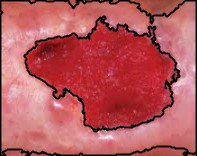
\includegraphics[keepaspectratio, width=3cm]{gambar/Bab4/Luka_merah_interpolasi.jpg}
		\caption{\textit{Border following}}
	\end{subfigure}
	\begin{subfigure}{.4\textwidth}
		\centering
		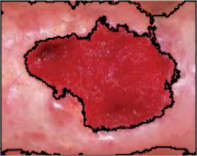
\includegraphics[keepaspectratio, width=3cm]{gambar/Bab4/Luka_merah_Globalinterpolasi.jpg}
		\caption{Hasil interpolasi}
	\end{subfigure} 
	\caption{Hasil Interpolasi dari deteksi \textit{border following}}
\end{figure}

Dari metode yang dipakai di atas, hanya didapatkan 
titik kontrol dari suatu kurva. Untuk mendapatkan 
kurva halus seperti yang dicanangkan dalam buku 
yang akan menghasilkan gambar(\ref{gambar:kurvaluka})
\textit{NURBS} dipakai algoritma dari Bézier(\ref{algoritma:bezier})
\begin{figure}[H]
	\centering
	\begin{lstlisting}[language=Python, basicstyle=\tiny]
		bernstein = lambda n, k, t: binom(n,k)* t**k * (1.-t)**(n-k)

		def bezier(points, num=400):
			N = len(points)
			t = np.linspace(0, 1, num=num)
			curve = np.zeros((num, 2))
			for i in range(N):
				curve += np.outer(GlobalInterpolation.bernstein(N - 1, i, t), points[i])
			return curve
	\end{lstlisting}
	\caption{Kode Bézier}
	\label{kode:bezier}
\end{figure}
\begin{figure}[H]
	\centering
	\begin{subfigure}{.3\textwidth}
		\centering
		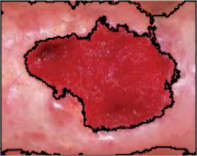
\includegraphics[keepaspectratio, width=3cm]{gambar/Bab4/Luka_merah_Globalinterpolasi.jpg}
		\caption{Interpolasi global}
	\end{subfigure}
	\begin{subfigure}{.4\textwidth}
		\centering
		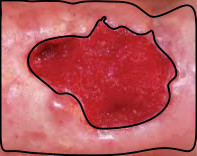
\includegraphics[keepaspectratio, width=3cm]{gambar/Bab4/Luka_merah_curve.jpg}
		\caption{Kurva bézier}
	\end{subfigure} 
	\caption{Penghalusan kurva menggunakan bézier}
	\label{gambar:kurvaluka}
\end{figure}
Kekurangan dari kode ini adalah kode ini tidak bisa diberi 
titik data yang banyak, sehingga penulis membataskan titik data 
menjadi 1000 dengan memotong titik data secara rata.

\section{Validasi}

Source image eksperimen diambil dari repository yang dapat diakses di
\href{https://github.com/mekas/InjuryDetection}{https://github.com/mekas/InjuryDetection}. 
Dari semua metode yang sudah ditunjukan 
dalam bab ini, maka akan dijalankan ke semua citra yang 
berada dalam repository. 

Dalam pengolahan citra, tidak semua citra dapat dipindai 
dengan baik. Apabila suatu pindaian dekat dengan bentuk 
\textit{ground truth} maka akan dikategorikan sebagai 
berhasil dan yang sebaliknya akan dikategorikan sebagai 
gagal seperti yang ditunjukan pada gambar(\ref{suksesgagal}). 
Hasil dari pindaian akan dimasukkan kedalam lampiran.
\begin{figure}[H]
	\centering
	\begin{subfigure}{.3\textwidth}
		\centering
		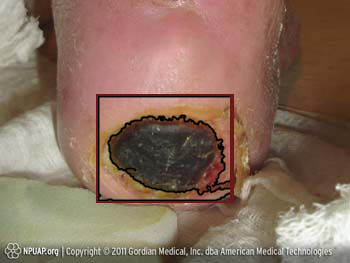
\includegraphics[keepaspectratio, width=3cm]{gambar/Data/BorderFollowing/Hitam/6 - failed.jpg}
		\caption{Gagal}
	\end{subfigure}
	\begin{subfigure}{.4\textwidth}
		\centering
		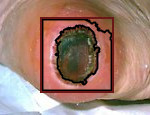
\includegraphics[keepaspectratio, width=3cm]{gambar/Data/BorderFollowing/Hitam/7 - sukses.jpg}
		\caption{Berhasil}
	\end{subfigure} 
	\caption{Alat validasi}
	\label{suksesgagal}
\end{figure}

Dalam memvalidasi citra, akan digunakan 
\textit{GIMP} dengan menggunakan \textit{fuzzy select tool} 
dengan treshold 75.- dan 2px feather edges lalu dilihat 
\textit{pixel count} nya dengan menggunakan \textit{histogram}. 
Karena program yang penulis pakai hanya memberi garis luar, maka 
daerah yang terdeteksi akan dihitamkan manual agar dapat 
dihitung luasnya. Setelah mendapatkan luas dari sumber data, 
maka akan dibandingkan dengan \textit{ground truth} menggunakan 
rumus(\ref{rumus:groundtruth})
\begin{figure}[H]
	\centering
	\begin{subfigure}{.3\textwidth}
		\centering
		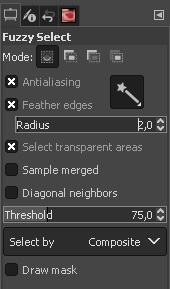
\includegraphics[keepaspectratio, width=3cm]{gambar/Bab4/fuzzyselect.jpg}
		\caption{\textit{fuzzyselect tool}}
	\end{subfigure}
	\begin{subfigure}{.4\textwidth}
		\centering
		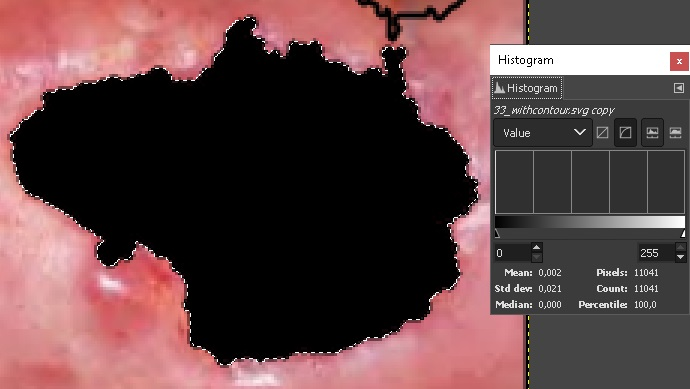
\includegraphics[keepaspectratio, width=3cm]{gambar/Bab4/histogram.jpg}
		\caption{\textit{histogram}}
	\end{subfigure} 
	\caption{Alat validasi}
\end{figure}

Percobaan dimulai dengan luka merah, didapatkan hasil sebagai berikut.
\begin{longtable}[width = 8cm]{| c | c | c | c | c |}
	\caption{Percobaan pada luka merah}
	\\
	\hline
	Indeks & Sumber & \textit{Border Following} & Interpolasi & \textit{Ground Truth}
	\endhead
	\hline\hline
	\multicolumn{5}{|c|}
	{Luka Merah}
	\\
	\hline\hline
	12 &
    \includegraphics[keepaspectratio, width=2cm]
    {Skripkating/Rizki_Wound_ACM/dataset_3/luka_merah/ready/12.jpg} &
    \includegraphics[keepaspectratio, width=2cm]
    {gambar/Data/BorderFollowing/Merah/12.jpg} &
    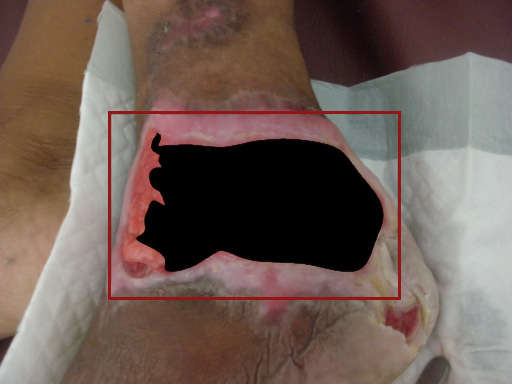
\includegraphics[keepaspectratio, width=2cm]
    {gambar/Data/Curve/Merah/12.jpg} &
    \includegraphics[keepaspectratio, width=2cm]
    {Skripkating/Rizki_Wound_ACM/dataset_3/luka_merah/ready/12_r.jpg}
	\\
	\hline
	18 &
    \includegraphics[keepaspectratio, width=2cm]
    {Skripkating/Rizki_Wound_ACM/dataset_3/luka_merah/ready/18.jpg} &
    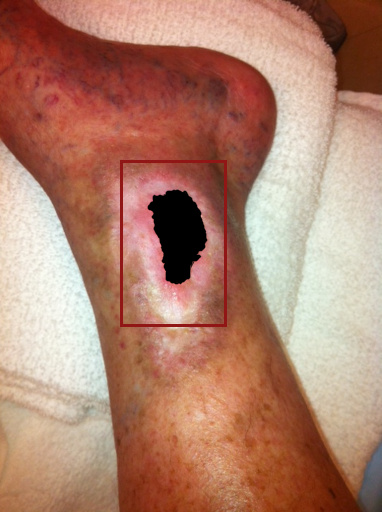
\includegraphics[keepaspectratio, width=2cm]
    {gambar/Data/BorderFollowing/Merah/18.jpg} &
    \includegraphics[keepaspectratio, width=2cm]
    {gambar/Data/Curve/Merah/18.jpg} &
    \includegraphics[keepaspectratio, width=2cm]
    {Skripkating/Rizki_Wound_ACM/dataset_3/luka_merah/ready/18_r.jpg}
	\\
	\hline
	33 &
    \includegraphics[keepaspectratio, width=2cm]
    {Skripkating/Rizki_Wound_ACM/dataset_3/luka_merah/ready/33.jpg} &
    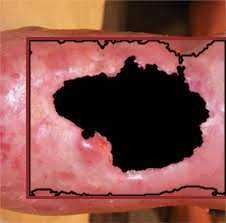
\includegraphics[keepaspectratio, width=2cm]
    {gambar/Data/BorderFollowing/Merah/33.jpg} &
    \includegraphics[keepaspectratio, width=2cm]
    {gambar/Data/Curve/Merah/33.jpg} &
    \includegraphics[keepaspectratio, width=2cm]
    {Skripkating/Rizki_Wound_ACM/dataset_3/luka_merah/ready/33_r.jpg}
	\\
	\hline
	44 &
    \includegraphics[keepaspectratio, width=2cm]
    {Skripkating/Rizki_Wound_ACM/dataset_3/luka_merah/ready/44.jpg} &
    \includegraphics[keepaspectratio, width=2cm]
    {gambar/Data/BorderFollowing/Merah/44.jpg} &
    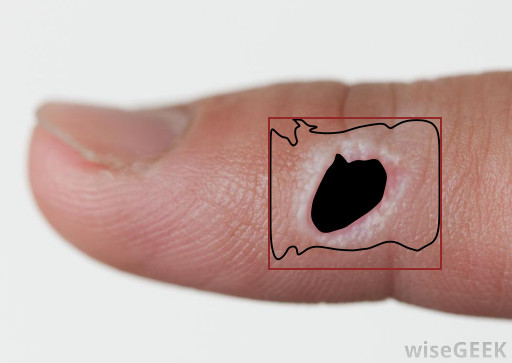
\includegraphics[keepaspectratio, width=2cm]
    {gambar/Data/Curve/Merah/44.jpg} &
    \includegraphics[keepaspectratio, width=2cm]
    {Skripkating/Rizki_Wound_ACM/dataset_3/luka_merah/ready/44_r.jpg}
	\\
	\hline
\end{longtable}
\begin{longtable}[width = 6cm]{| c | c | c | c | c | c |}
    \caption{Similiaritas deteksi luka merah \textit{border following} 
    dan yang dibantu dengan interpolasi}
    \\
    \hline  
    \multicolumn{6}{|c|}{Luka Merah}
    \\
    \hline
    Indeks & \textbf{GT}(px) & \textbf{BF}(px) & Similiaritas($\%$) & Intp(px) & Similiaritas($\%$)
    \endhead
    \hline  12&	29834&	26565&	89.04270296&	26182&	87.75893276 \\
    \hline  18&	2788&	3596&	71.01865136&	3337&	80.30846485 \\
    \hline  33&	10951&	11176&	97.94539311&	10732&	98.00018263 \\
    \hline  44&	2395&	4172&	25.80375783&	3966&	34.40501044 \\
    \hline  \multicolumn{2}{|c|}{}& \textit{Average}&    70.95262632&    \textit{Average}&    75.11814767 \\
    \hline
\end{longtable}
\begin{itemize}
    \setlength{\itemsep}{0pt}
    \setlength{\parskip}{0pt}
    \setlength{\parsep}{0pt}
    \item GT = \textit{Ground Truth}
    \item BF = \textit{Border Following}
    \item Intp = Interpolasi
\end{itemize}
\begin{itemize}
    \setlength{\itemsep}{0pt}
    \setlength{\parskip}{0pt}
    \setlength{\parsep}{0pt}
    \item Jumlah luka merah = 30
    \item Jumlah luka yang terdeteksi contour tracing = 4
\end{itemize}
Dari percobaan deteksi luka merah, tingkat pendeteksian 
dari \textit{border following} lumayan rendah, terdapat 4 
pindaian yang berhasil dari 30 citra, namun memiliki 
similiaritas yang bagus terhadap \textit{ground truth}, dan 
Bantuan dari Interpolasi meningkatkan similiaritas 
sebesar 4.16$\%$. 

Percobaan akan dilanjut ke luka kuning.
\begin{longtable}[width = 8cm]{| c | c | c | c | c |}
	\caption{Percobaan pada luka kuning}
	\\
	\hline
	Indeks & Sumber & \textit{Border Following} & Interpolasi & \textit{Ground Truth}
	\endhead
	\hline\hline
	\multicolumn{5}{|c|}
	{Luka Kuning}
	\\
	\hline\hline
	17 &
    \includegraphics[keepaspectratio, width=2cm]
    {Skripkating/Rizki_Wound_ACM/dataset_3/luka_kuning/ready/17.jpg} &
    \includegraphics[keepaspectratio, width=2cm]
    {gambar/Data/BorderFollowing/Kuning/17.jpg} &
    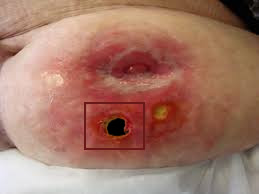
\includegraphics[keepaspectratio, width=2cm]
    {gambar/Data/Curve/Kuning/17.jpg} &
    \includegraphics[keepaspectratio, width=2cm]
    {Skripkating/Rizki_Wound_ACM/dataset_3/luka_kuning/ready/17_r.jpg}
	\\
	\hline
	25 &
    \includegraphics[keepaspectratio, width=2cm]
    {Skripkating/Rizki_Wound_ACM/dataset_3/luka_kuning/ready/25.jpg} &
    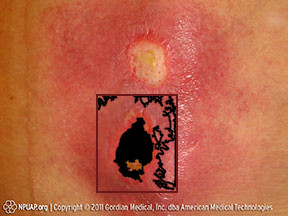
\includegraphics[keepaspectratio, width=2cm]
    {gambar/Data/BorderFollowing/Kuning/25.jpg} &
    \includegraphics[keepaspectratio, width=2cm]
    {gambar/Data/Curve/Kuning/25.jpg} &
    \includegraphics[keepaspectratio, width=2cm]
    {Skripkating/Rizki_Wound_ACM/dataset_3/luka_kuning/ready/25_r.jpg}
	\\
	\hline
\end{longtable}
\begin{longtable}[width = 6cm]{| c | c | c | c | c | c |}
    \caption{Similiaritas deteksi luka kuning \textit{border following} 
    dan yang dibantu dengan interpolasi}
    \\
    \hline  
    \multicolumn{6}{|c|}{Luka Kuning}
    \\
    \hline
    Indeks & \textbf{GT}(px) & \textbf{BF}(px) & Similiaritas($\%$) & Intp(px) & Similiaritas($\%$)
    \endhead
    \hline  17&	319&	317&	99.37304075&	282&	88.40125392 \\
    \hline  25&	2831&	1345&	47.50971388&	1291&	45.60226069 \\
    \hline  \multicolumn{2}{|c|}{}& \textit{Average}&    73.44137732&    \textit{Average}&    67.0017573 \\
    \hline
\end{longtable}
\begin{itemize}
    \setlength{\itemsep}{0pt}
    \setlength{\parskip}{0pt}
    \setlength{\parsep}{0pt}
    \item GT = \textit{Ground Truth}
    \item BF = \textit{Border Following}
    \item Intp = Interpolasi
\end{itemize}
\begin{itemize}
    \setlength{\itemsep}{0pt}
    \setlength{\parskip}{0pt}
    \setlength{\parsep}{0pt}
    \item Jumlah luka kuning = 15
    \item Jumlah luka yang terdeteksi contour tracing = 2
\end{itemize}
Setelah melakukan percobaan di luka kuning, dapat dilihat 
tingkat pendeteksian masih sama seperti pada luka merah, yaitu 
13.3$\%$, namun mendapat peningkatan pada pengecekan similiaritas 
di \textit{border following} pada angka 73.4$\%$, tetapi terjadi 
penurunan 6.43$\%$ di bantuan interpolasi terhadap \textit{border following}

Kategori terakhir untuk dipercobakan adalah luka hitam.
\begin{longtable}[width = 8cm]{| c | c | c | c | c |}
	\caption{Percobaan pada luka hitam}
	\\
	\hline
	Indeks & Sumber & \textit{Border Following} & Interpolasi & \textit{Ground Truth}
	\endhead
	\hline\hline
	\multicolumn{5}{|c|}
	{Luka Hitam}
	\\
	\hline\hline
	7 &
    \includegraphics[keepaspectratio, width=2cm]
    {Skripkating/Rizki_Wound_ACM/dataset_3/luka_hitam/ready/7.jpg} &
    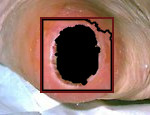
\includegraphics[keepaspectratio, width=2cm]
    {gambar/Data/BorderFollowing/Hitam/7.jpg} &
    \includegraphics[keepaspectratio, width=2cm]
    {gambar/Data/Curve/Hitam/7.jpg} &
    \includegraphics[keepaspectratio, width=2cm]
    {Skripkating/Rizki_Wound_ACM/dataset_3/luka_hitam/ready/7_r.jpg}
	\\
	\hline
	18 &
    \includegraphics[keepaspectratio, width=2cm]
    {Skripkating/Rizki_Wound_ACM/dataset_3/luka_hitam/ready/18.jpg} &
    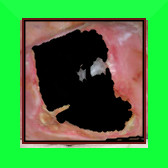
\includegraphics[keepaspectratio, width=2cm]
    {gambar/Data/BorderFollowing/Hitam/18.jpg} &
    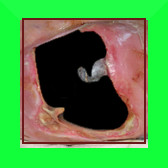
\includegraphics[keepaspectratio, width=2cm]
    {gambar/Data/Curve/Hitam/18.jpg} &
    \includegraphics[keepaspectratio, width=2cm]
    {Skripkating/Rizki_Wound_ACM/dataset_3/luka_hitam/ready/18_r.jpg}
	\\
	\hline
	26 &
    \includegraphics[keepaspectratio, width=2cm]
    {Skripkating/Rizki_Wound_ACM/dataset_3/luka_hitam/ready/26.jpg} &
    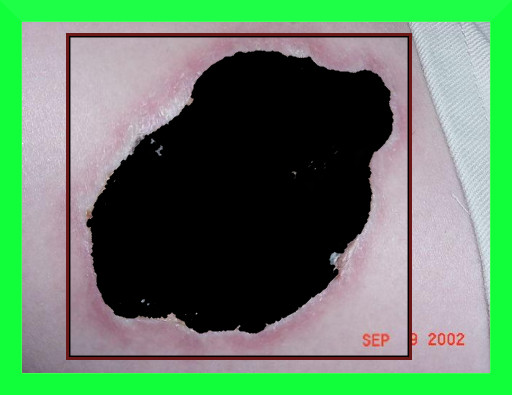
\includegraphics[keepaspectratio, width=2cm]
    {gambar/Data/BorderFollowing/Hitam/26.jpg} &
    \includegraphics[keepaspectratio, width=2cm]
    {gambar/Data/Curve/Hitam/26.jpg} &
    \includegraphics[keepaspectratio, width=2cm]
    {Skripkating/Rizki_Wound_ACM/dataset_3/luka_hitam/ready/26_r.jpg}
	\\
	\hline
	28 &
    \includegraphics[keepaspectratio, width=2cm]
    {Skripkating/Rizki_Wound_ACM/dataset_3/luka_hitam/ready/28.jpg} &
    \includegraphics[keepaspectratio, width=2cm]
    {gambar/Data/BorderFollowing/Hitam/28.jpg} &
    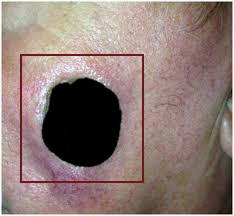
\includegraphics[keepaspectratio, width=2cm]
    {gambar/Data/Curve/Hitam/28.jpg} &
    \includegraphics[keepaspectratio, width=2cm]
    {Skripkating/Rizki_Wound_ACM/dataset_3/luka_hitam/ready/28_r.jpg}
	\\
	\hline
	29 &
    \includegraphics[keepaspectratio, width=2cm]
    {Skripkating/Rizki_Wound_ACM/dataset_3/luka_hitam/ready/29.jpg} &
    \includegraphics[keepaspectratio, width=2cm]
    {gambar/Data/BorderFollowing/Hitam/29.jpg} &
    \includegraphics[keepaspectratio, width=2cm]
    {gambar/Data/Curve/Hitam/29.jpg} &
    \includegraphics[keepaspectratio, width=2cm]
    {Skripkating/Rizki_Wound_ACM/dataset_3/luka_hitam/ready/29_r.jpg}
	\\
	\hline
	33 &
    \includegraphics[keepaspectratio, width=2cm]
    {Skripkating/Rizki_Wound_ACM/dataset_3/luka_hitam/ready/33.jpg} &
    \includegraphics[keepaspectratio, width=2cm]
    {gambar/Data/BorderFollowing/Hitam/33.jpg} &
    \includegraphics[keepaspectratio, width=2cm]
    {gambar/Data/Curve/Hitam/33.jpg} &
    \includegraphics[keepaspectratio, width=2cm]
    {Skripkating/Rizki_Wound_ACM/dataset_3/luka_hitam/ready/33_r.jpg}
	\\
	\hline
	40 &
    \includegraphics[keepaspectratio, width=2cm]
    {Skripkating/Rizki_Wound_ACM/dataset_3/luka_hitam/ready/40.jpg} &
    \includegraphics[keepaspectratio, width=2cm]
    {gambar/Data/BorderFollowing/Hitam/40.jpg} &
    \includegraphics[keepaspectratio, width=2cm]
    {gambar/Data/Curve/Hitam/40.jpg} &
    \includegraphics[keepaspectratio, width=2cm]
    {Skripkating/Rizki_Wound_ACM/dataset_3/luka_hitam/ready/40_r.jpg}
	\\
	\hline
	41 &
    \includegraphics[keepaspectratio, width=2cm]
    {Skripkating/Rizki_Wound_ACM/dataset_3/luka_hitam/ready/41.jpg} &
    \includegraphics[keepaspectratio, width=2cm]
    {gambar/Data/BorderFollowing/Hitam/41.jpg} &
    \includegraphics[keepaspectratio, width=2cm]
    {gambar/Data/Curve/Hitam/41.jpg} &
    \includegraphics[keepaspectratio, width=2cm]
    {Skripkating/Rizki_Wound_ACM/dataset_3/luka_hitam/ready/41_r.jpg}
	\\
	\hline
\end{longtable}
\begin{longtable}[width = 6cm]{| c | c | c | c | c | c |}
    \caption{Similiaritas deteksi luka hitam \textit{border following} 
    dan yang dibantu dengan interpolasi}
    \\
    \hline  
    \multicolumn{6}{|c|}{Luka Hitam}
    \\
    \hline
    Indeks & \textbf{GT}(px) & \textbf{BF}(px) & Similiaritas($\%$) & Intp(px) & Similiaritas($\%$)
    \endhead
    \hline  7&	2146&	2061&	96.03914259&	1928&	89.8415657  \\
    \hline  18&	7328&	6430&	87.74563319&	6009&	82.00054585 \\
    \hline  26&	60411&	60923&	99.15247223&	59143&	97.90104451 \\
    \hline  28&	5408&	5608&	96.30177515&	5902&	90.86538462 \\
    \hline  29&	43763&	44984&	97.20997189&	43368&	99.09741106 \\
    \hline  33&	12899&	9792&	75.91286146&	9417&	73.00565935 \\
    \hline  40&	3040&	3069&	99.04605263&	2948&	96.97368421 \\
    \hline  41&	9644&	9466&	98.15429282&	9365&	97.10700954 \\
    \hline  \multicolumn{2}{|c|}{}& \textit{Average}&    92.5807947&    \textit{Average}&    91.54594104 \\
    \hline
\end{longtable}
\begin{itemize}
    \setlength{\itemsep}{0pt}
    \setlength{\parskip}{0pt}
    \setlength{\parsep}{0pt}
    \item GT = \textit{Ground Truth}
    \item BF = \textit{Border Following}
    \item Intp = Interpolasi
\end{itemize}
\begin{itemize}
    \setlength{\itemsep}{0pt}
    \setlength{\parskip}{0pt}
    \setlength{\parsep}{0pt}
    \item Jumlah luka hitam = 24
    \item Jumlah luka yang terdeteksi contour tracing = 8
\end{itemize}
Percobaan terakhir terhadap luka hitam terdapat 
peningkatan pada tingkat deteksi, berada di angka 
33.3$\%$. Similiaritas juga terjadi peningkatan yaitu 
menjadi 92.6$\%$ dan terjadi penurunan yang similiar pada 
deteksi dengan bantuan interpolasi sebesar 2.85$\%$.

Dari hasil tes, didapatkan hasil merupakan berikut:
\begin{itemize}
	\item Hasil deteksi pada luka merah menghasilkan 4 
	citra yang terdeteksi dari 30 citra  akurasi daerah luas 
	kurva 70.9$\%$ pada \textit{border following} 
	dan 75.1$\%$ setelah di-interpolasi
	\item Hasil deteksi pada luka kuning menghasilkan 2 
	citra yang terdeteksi dari 15 citra  akurasi daerah luas 
	kurva 73.4$\%$ pada \textit{border following} 
	dan 67$\%$ setelah di-interpolasi
	\item Hasil deteksi pada luka hitam menghasilkan 8 
	citra yang terdeteksi dari 24	 citra  akurasi daerah luas 
	kurva 92.6$\%$ pada \textit{border following} 
	dan 91.5$\%$ setelah di-interpolasi
\end{itemize}
Dari hasil ini, dapat dilihat bahwa interpolasi spline 
yang dilakukan sering sekali menurunkan angka similiaritas 
di hasil tes pendeteksian luka. Penulis menspekulasi penyebab 
dari penurunan ini dikarenakan interpolasi memindahkan titik 
data yang diberikan oleh alat deteksi, \textit{border following} 
yang sudah berada dekat di garis \textit{ground truth} dipindah 
secara sembarang dimana lebih sering menjauh daripada mendekat.



% Baris ini digunakan untuk membantu dalam melakukan sitasi
% Karena diapit dengan comment, maka baris ini akan diabaikan
% oleh compiler LaTeX.
\begin{comment}
\bibliography{daftar-pustaka}
\end{comment}
